%----------------------------------------------------------------------------------------
%	PACKAGES AND THEMES
%----------------------------------------------------------------------------------------
\documentclass[aspectratio=169,xcolor=dvipsnames]{beamer}
\usetheme{Simple}

\usefonttheme[onlymath]{serif}

\usepackage{xcolor}
\usepackage{marvosym}
\usepackage{amsmath}
\usepackage{hyperref}
\usepackage{graphicx} % Allows including images
\usepackage{booktabs} % Allows the use of \toprule, \midrule and \bottomrule in tables
\usepackage{braket}

\newcommand{\pder}[2]{\frac{\partial #1}{\partial #2}}
\newcommand{\dt}{\frac{d}{dt}}
\newcommand{\dder}[2]{\frac{d#1}{d#2}}
\newcommand{\horrule}[1]{\rule{\linewidth}{#1}} 
\newcommand{\overbar}[1]{
	\mkern 1.5mu \overline{\mkern-1.5mu\raisebox{0pt}[\dimexpr\height+0.5mm\relax]{$#1$}\mkern-1.5mu}\mkern 1.5mu
}
\newcommand*\dif{\mathop{}\!\mathrm{d}}
\newcommand{\expval}[1]{\langle #1 \rangle}
\newcommand{\tr}{\text{Tr }}

%----------------------------------------------------------------------------------------
%	TITLE PAGE
%----------------------------------------------------------------------------------------

\title[short title]{Parton Distribution Functions} % The short title appears at the bottom of every slide, the full title is only on the title page
\subtitle{arXiv:hep-lat/9609018 }

\author[Youngwan Kim] {Youngwan Kim}

\institute[SNUCMS] % Your institution as it will appear on the bottom of every slide, may be shorthand to save space
{
	Seoul National University\vskip0.05in
	SNUCMS arXiv Seminar
     % Your institution for the title page
    \vskip 3pt
}
\date{\today} % Date, can be changed to a custom date


%----------------------------------------------------------------------------------------
%	PRESENTATION SLIDES
%----------------------------------------------------------------------------------------

\begin{document}

\begin{frame}
    % Print the title page as the first slide
    \titlepage
\end{frame}

\begin{frame}
	\frametitle{Outline}
	\tableofcontents
\end{frame}

%------------------------------------------------
\section{Introduction to PDFs}
%------------------------------------------------
\subsection{Intuition to PDFs}

\begin{frame}{Intution to PDFs}
	  \begin{columns}[T]
		\begin{column}{.5\textwidth}
				\centering
				\begin{figure}
					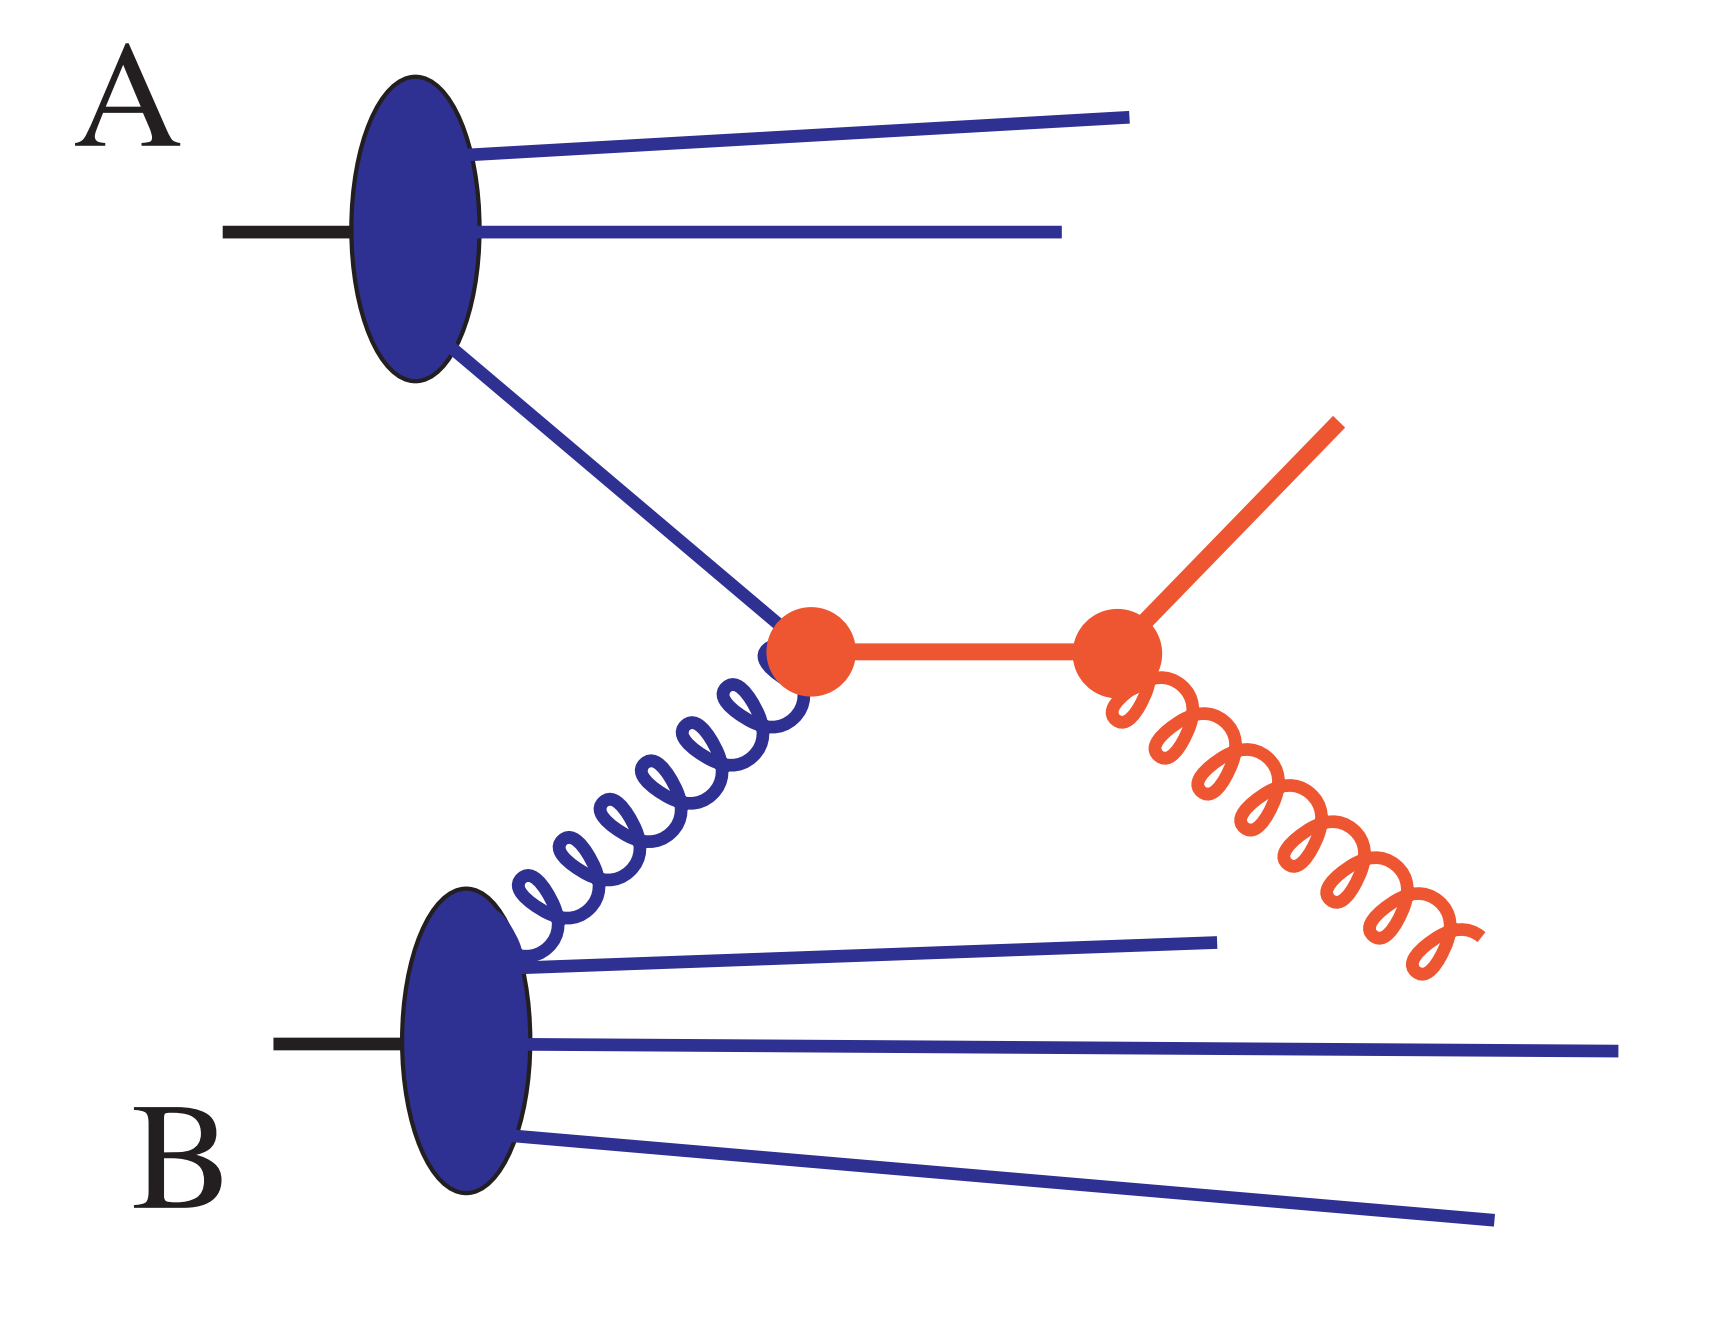
\includegraphics[width=0.9\textwidth]{parton.png}
					\caption{Hadron A + Hadron B $\to$ 2 partons}
				\end{figure}
		\end{column}
		\centering 
		\begin{column}{.45\textwidth}
			Consider a collision of two hadrons A and B... \vskip0.1in
			\begin{itemize}
				\item parton $a$ from hadron $A$ with $\xi_A$ fraction of its momentum
				\vskip0.05in
				\setbeamertemplate{itemize items}[triangle]
				\begin{itemize}
					\item $f_{a/A}(\xi_A)\dif \xi_A$
				\end{itemize}\vskip0.075in
				\setbeamertemplate{itemize items}[circle]
				\item parton $b$ from hadron $B$ with $\xi_B$ fraction of its momentum
				\vskip0.05in
				\setbeamertemplate{itemize items}[triangle]
				\begin{itemize}
					\item $f_{b/B}(\xi_A)\dif \xi_B$
				\end{itemize}\vskip0.075in
				\setbeamertemplate{itemize items}[circle]
				\item \alert{$\dif \hat{\sigma}$} parton level cross section
			\end{itemize}\vskip0.1in
			One can describe $\dif \sigma$ as a product of these three factors...
		\end{column}
	\end{columns}
\end{frame}

\subsection{Factorization}
\begin{frame}{Factorization}
	\begin{block}{Hadron Scattering Cross Section}
		\centering
		\begin{align*}
			\dder{\sigma}{p_T} \sim \sum_{a,b}\int \dif \xi_A f_{a/A}(\xi_A,\mu) \int  \dif \xi_B f_{b/B}(\xi_B,\mu) \dder{\hat{\sigma}}{p_T}
		\end{align*}
	\end{block}

	\begin{block}{Parton Level Cross Section}
		\centering
		\begin{align*}
			 \dder{\hat{\sigma}}{p_T} \sim \sum_N \left( \frac{\alpha_S(\mu)}{\pi} \right)^N H_N\left(\xi_A,\xi_B,p_T;a,b,\mu\right)
		\end{align*}
	\end{block}\vskip0.15in

	\begin{itemize}
		\item The coefficients $H_N$ are calculable via pQCD ; regard factorization as an established theorem of QCD
	\end{itemize}
\end{frame}

\begin{frame}{Factorization}
	Another parameter $\mu$? : there is more to the equation than just a model\vskip0.15in
	\begin{itemize}
		\item Has dimension of mass $\to$ renormalization of $\alpha_S(\mu)$ and $f_{a/A}(\xi_A)$
		\item $\dif \hat{\sigma} / \dif p_T$ is calculated straightforwardly at Born level\vskip0.075in
		\setbeamertemplate{itemize items}[triangle]
		\begin{itemize}
			\item Divergences appear starting from NLO and beyond, calculation gets tricky\vskip0.05in
			\item Such divergences are removed, and in their place dependence of the scale $\mu$ appears.
		\end{itemize}
	\end{itemize}
\end{frame}

\subsection{Significance of PDFs}
\begin{frame}{Significance of PDFs}
	\vskip0.1in
	Knowledge of PDFs is necessary for the description of hard processes, \vskip0.1in
	\begin{block}{Parton-Parton Cross Section (ex. LHC, Fermilab)}
		\begin{align*}
		\dif\sigma \sim \sum_{a,b}\int \dif \xi_A f_{a/A}(\xi_A,\mu) \int  \dif \xi_B f_{b/B}(\xi_B,\mu) \dif\hat{\sigma}
	\end{align*}
	\end{block}\vskip0.05in
	\begin{block}{DIS Cross Section (ex. HERA)}
		\begin{align*}
			\dif\sigma \sim \sum_{a}\int \dif \xi_A f_{a/A}(\xi_A,\mu) \dif\hat{\sigma}
		\end{align*}
	\end{block}\vskip0.1in
	Obvious as no prediction is available without any knowledge of PDFs.
\end{frame}

\begin{frame}{Significance of PDFs}
	For both expressions of $\dif\sigma$ it shows that in high energy, short distance collisions...\vskip0.1in
	\begin{itemize}
		\item a hard scattering probes the system quickly 
		\item strong binding forces act slowly
	\end{itemize} \vskip0.15in
	\MVRightarrow{} One needs to know probabilities to find partons in a \textbf{fast moving} hadron as seen by an approximately instantaneous probe \vskip0.1in
	\MVRightArrow{} PDFs should provide a \textbf{relativistic} view of partons
\end{frame}

\section{Technical Definition of PDFs}

\subsection{Technical Definition of PDFs}
\begin{frame}{Technical Definition of PDFs}
	%Will define PDFs in terms of field operators along a light-like line \vskip0.15in
	\begin{itemize}
		\item Coordinates : $x^\pm = (x^0 \pm x^3)/\sqrt{2}$ ,  $P^\pm = (P^0 \pm P^3)/\sqrt{2}$ , $v=(v^+,v^-,\mathbf{v_T})$
	\end{itemize}\vskip0.1in
	\begin{columns}[T]
		\begin{column}{.4\textwidth}
		\centering
			\begin{figure}
				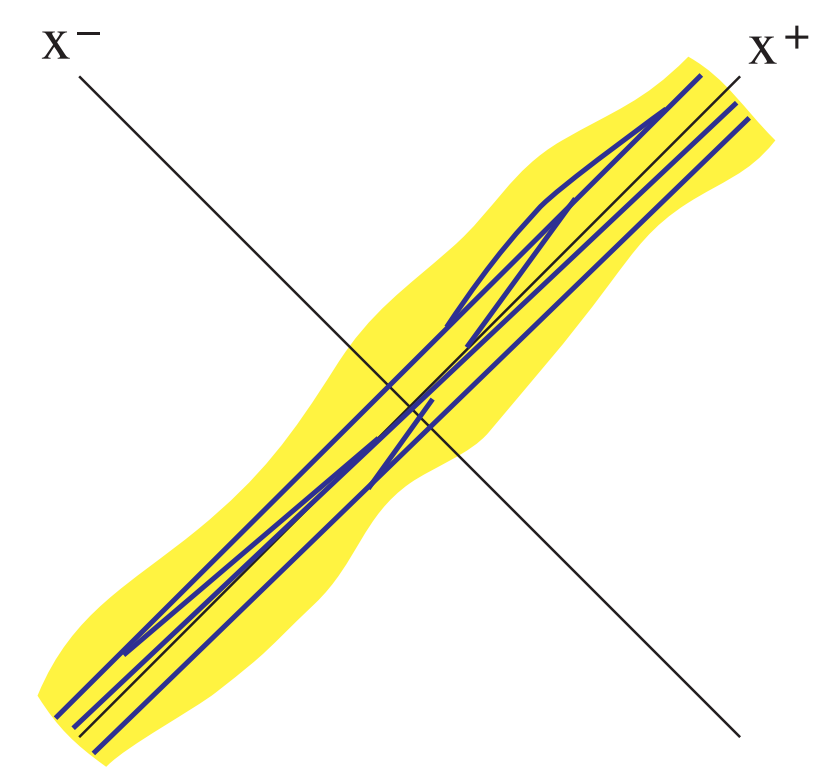
\includegraphics[width=0.75\textwidth]{worldline.png}
				\caption{partons in a fast moving proton}
			\end{figure}
		\end{column}
		\begin{column}{.5\textwidth}
			\setbeamertemplate{itemize items}[triangle]
			\begin{itemize}
				\item $x^+$ can be interpreted as time \vskip 0.15in
				\item partons in a proton with a small $P^-$, big $P^+$ and $\vec{P_T}=0$, move roughly parallel to the $x^+$ axis.\vskip0.15in
				\item PDFs are to be defined via \textbf{null plane field theory}, a field theory quantized on planes of equal $x^+$.
				\item $P^\mu x_\mu = P^+ x^- +P^- x^+ - \mathbf{P_T}\cdot \mathbf{x_T}$\vskip0.15in
			\end{itemize}
		\end{column}
	\end{columns}
\end{frame}

\begin{frame}{Technical Definition of PDFs}
	We want to define $f_{i/A}(\xi,\mu)$, the probability density for ... \vskip0.1in
	\begin{itemize}
		\item finding a parton of flavor $i$ (quark, antiquark, gluon ...) 
		\item which carries a fraction $\xi$ of $P^+$
		\item in the hadron $A$ with momentum $P$.
	\end{itemize}\vskip0.15in
	\MVRightArrow{} Approach by defining a \textbf{density operator} using creation, annihilation operators of null plane field theory
\end{frame}

\begin{frame}{Technical Definition of PDFs}
	Consider $b(\xi P^+, \mathbf{k_T},s,c;i)$ which annihilates ($b^\dagger$ creates)
	\begin{itemize}
		\item a quark with flavor $i$, having helicity $s$ and color $c$
		\item carrying a fraction $\xi$ of $P^+$ of the proton with transverse momentum $\mathbf{k_T}$
		\item $b(\xi P^+, \mathbf{k_T},s,c;i) \ket{0} = 0$ for the vacuum state $\ket{0}$
		\item normalized by the following anticommutation relation :
	\end{itemize}\vskip0.1in
	\begin{block}{Anticommutation relation of $b$,$b^\dagger$}
		\begin{align*}
			   \left\{ b(\xi' P^+, \mathbf{k_T'},s',c';i),b(\xi P^+, \mathbf{k_T},s,c;i)\right\}   = (2\pi)^3 2\xi P^+ \delta(\xi'P^+ - \xi P^+)\delta(\mathbf{k_T'}-\mathbf{k_T})\delta_{s',s} \delta_{c',c} \\
		\end{align*}
	\end{block}
\end{frame}

\begin{frame}{Technical Definition of PDFs}
	With $b$ and $b^\dagger$, one could define $\rho(\xi P^+,\mathbf{k_T};i)$ which \textbf{counts the number of quarks} in  a region of $\xi$ and $\mathbf{k_T}$\vskip0.1in
	\begin{block}{Definition of $\rho$}
		\begin{align*}
		\rho(&\xi P^+,\mathbf{k_T};i)  \\
		&= \frac{1}{(2\pi)^3 2\xi} \sum_{s,c}b^\dagger(\xi P^+, \mathbf{k_T},s,c;i)b(\xi P^+, \mathbf{k_T},s,c;i) \\
		\end{align*}
\end{block}
\end{frame}

\begin{frame}{Technical Definition of PDFs}
	If $\ket{\Psi}$ is obtained by applying $b$ to the vacuum, $\rho$ counts the number $N(\mathcal{V})$ of quarks in the momentum-space volume $\mathcal{V}$ when integrated,
	\begin{align*}
		\int_\mathcal{V} \dif\xi \dif \mathbf{k_T} \rho(&\xi P^+,\mathbf{k_T};i) \ket{\Psi} = N(\mathcal{V}) \ket{\Psi}
	\end{align*}
	
	Here we can take a matrix element of $\rho$ in a proton state to define $f_{i/A}(\xi)$\vskip0.1in
	\begin{block}{Preliminary definition of $f_{i/A}(\xi)$ I}
		\begin{align*}
			f_{i/A}(\xi) \braket{P'|P} = \int \dif\mathbf{k_T} \braket{P'|\rho(\xi P^+,\mathbf{k_T};i)|P}\\
		\end{align*}
	\end{block}
\end{frame}

\begin{frame}{Technical Definition of PDFs}
	In order to make this construction more useful, we relate $b,b^\dagger$ with the quark field operator $\psi_i(x)$ quantized on the null plane as ...
	% The dynamical part of the quark field at $x^+=0$ is related to quark and antiquark creation and destruction operators by
	\begin{align*}
		P_{dy}&\psi_{i,c}(x^+=0,x^-,\mathbf{x_T}) = \frac{1}{(2\pi)^3} \int_{0}^{\infty} \frac{\dif k^+}{2k^+} \int \dif\mathbf{k_T} \\
		&\times \sum_s \left\{ \begingroup \color{red} P_{dy}u(k,s)\endgroup e^{-ik\cdot x}b(k^+, \mathbf{k_T},s,c;i)+\begingroup \color{red}P_{dy}v(k,s) \endgroup e^{+ik\cdot x}d^\dagger(k^+, \mathbf{k_T},s,c;i)\right\}
	\end{align*}
	\begin{itemize}
		\item The \alert{two components} projected by $P_{dy}=\frac{1}{2}\gamma^-\gamma^+$ are the independent dynamical fields representing quarks. 
		\item $u(k,s),v(k,s)$ : usual spinor solutions of the free Dirac eq, normalized to $\overbar{u}(k,s)\gamma^+ u(k,s)=2k^+$ (same with $v(k,s)$)
		\item $d^\dagger(k^+, \mathbf{k_T},s,c;i)$ : antiquark creation operator (analogous to $b^\dagger$)
	\end{itemize}
\end{frame}

\begin{frame}{Technical Definition of PDFs}
	Then plugging in the above expression into the preliminary definition of $f_{i/A}(\xi)$, \vskip0.15in
	\begin{block}{Preliminary definition of $f_{i/A}(\xi)$ II}
		\begin{align*}
		f_{i/A}(\xi)&\braket{P'|P}=\frac{P^+}{2\pi}\int \dif y^- e^{-i\xi P^+ y^-} \int \dif x^- d\mathbf{x_T} \\
		&\times \braket{P'|\overbar{\psi}_i(0,x^-+y^-,\mathbf{x_T})\gamma^+\psi_i(0,x^-,\mathbf{x_T})|P}\\
		\end{align*}
	\end{block}
	
\end{frame}

\begin{frame}{Technical Definition of PDFs}
		and implementing the following identities : \vskip0.05in
	\begin{itemize}
		\item Translation invariance : 
		\begin{align*}
			&\braket{P'|\overbar{\psi}_i(0,x^-+y^-,\mathbf{x_T})\gamma^+\psi_i(0,x^-,\mathbf{x_T})|P} \\
			&=\exp\left[i(P'-P)\cdot x^--(\mathbf{P'_T}-\mathbf{P_T})\cdot \mathbf{x_T} \right] \times \braket{P'|\overbar{\psi}_i(0,y^-,\mathbf{0})\gamma^+ \psi_i(\mathbf{0})|P}
		\end{align*} 
		\item Proton state normalization : $\braket{P'|P}=(2\pi)^3 2P^+ \delta(P'^+ - P^+) \delta(\mathbf{P'_T}-\mathbf{P_T})$
	\end{itemize}

	\begin{block}{Preliminary definition of $f_{i/A}(\xi)$}
		\begin{align*}
			f_{i/A}(\xi) = \frac{1}{4\pi} \int \dif y^- e^{-i\xi P^+ y^-} \braket{P|\overbar{\psi}_i(0,y^-,\mathbf{0})\gamma^+\psi_i(0)|P}\\
		\end{align*}
	\end{block}
\end{frame}

\begin{frame}{Technical Definition of PDFs}		
	
	\begin{block}{Preliminary definition of $f_{i/A}(\xi)$}
		\begin{align*}
		f_{i/A}(\xi) = \frac{1}{4\pi} \int \dif y^- e^{-i\xi P^+ y^-} \braket{P|\begingroup \color{red} \overbar{\psi}_i(0,y^-,\mathbf{0})\gamma^+\psi_i(0)\endgroup|P}\\
		\end{align*}
	\end{block}\vskip0.15in
				        
	Things to notice from $f_{i/A}(\xi)$ ... \vskip0.1in
	\begin{itemize}
		\item It is an expectation value in the hadron state of a certain \alert{operator}.
		\item This operator is not local but \textbf{bilocal} : $(0,y^-,\mathbf{0})$ and $(0,0,\mathbf{0})$ are light-like separated.
		\item Integrate over $y^-$ with the right factor so that we annihilate a quark with $\xi P^+$ momentum.
	\end{itemize}

	\MVRightArrow{} Gluons ...? Gauge invariance ...? Renormalization ...?
\end{frame}

\subsection{Gauge Invariance}
\begin{frame}{Gauge Invariance}
	The $f_{i/A}(\xi)$ above relies on the gluon potential $A^\mu$ being in the lightlike axial gauge $A^+=0$, so it would be nice to ...
	\begin{itemize}
		\item make the \alert{operator} gauge invariant
		\item match the previous definition in $A^+=0$ gauge
	\end{itemize}\vskip0.1in
	\MVRightArrow{} Solution : insert a Wilson line factor $\mathcal{O}$ into the operator 
	
	\begin{block}{Wilson line factor}
		\begin{align*}
			\mathcal{O}(y^-,0)=\mathcal{P}\exp \left[ ig \int_{0}^{y^-} \dif z^- A^+(0,z^-,\mathbf{0})_a t_a \right]
		\end{align*}
		\centering
		 $t_a$ : $SU(3)_c$ generator matrix in the $\mathbf{3}$ representation \vskip0.05in
		$\mathcal{P}$ : path ordering with more positive $y^-$ values to the left \vskip0.1in
 	\end{block}
	
\end{frame}

\begin{frame}{Gauge Invariance}
	Then the revised gauge invariant $f_{i/A}(\xi)$ is defined as :\vskip0.1in
	\begin{block}{Gauge invariant definition of $f_{i/A}(\xi)$}
		\begin{align*}
		f_{i/A}(\xi) = \frac{1}{4\pi} \int \dif y^- e^{-i\xi P^+ y^-} \braket{P|\begingroup \color{blue} \overbar{\psi}_i(0,y^-,\mathbf{0})\gamma^+\mathcal{O}(y^-,0)\psi_i(0)\endgroup|P}\\
		\end{align*}
	\end{block}\vskip0.15in

	one can immediately see that the gauge $A^+=0$ corresponds to $\mathcal{O}=1$, being consistent with the previous definition of $f_{i/A}(\xi)$
\end{frame}

\begin{frame}{Gauge Invariance}
	Checking gauge invariance under an unitary transformation $U(x)$ : 
	\begin{align*}
		\psi_i(0) &\to U(0)\psi_i(0) \\
		\overbar{\psi}_i(0,y^-,\mathbf{0}) &\to \overbar{\psi}_i(0,y^-,\mathbf{0}) U(0,y^-,\mathbf{0})^{-1} \\
		\mathcal{O}(y^-,0) &\to U(0,y^-,\mathbf{0})\mathcal{O}(y^-,0) U(0)^{-1}
	\end{align*}
	
	Thus including $\mathcal{O}(y^-,0)$, the \textcolor{blue}{operator} maintains invariant under a change of gauge. \vskip0.15in
	
	Besides gauge invariance what does $\mathcal{O}$ offer? Is there any physical significance ...? A mere technique?
\end{frame}



\begin{frame}{Gauge Invariance}
	\begin{columns}[T]
		\begin{column}{.5\textwidth}
			\begin{figure}
				\centering
				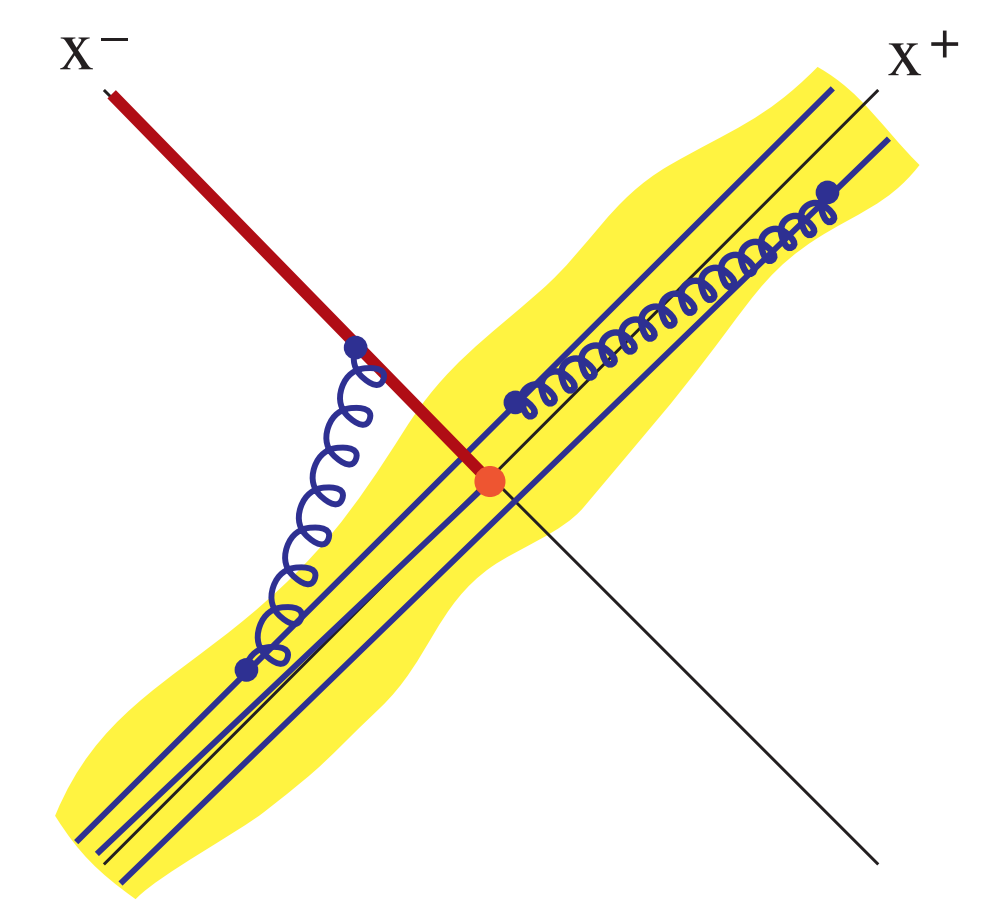
\includegraphics[width=.8\textwidth]{eikonal}
				\caption{Effect of the $\mathcal{O}$ operator}
			\end{figure}
		\end{column}
		\begin{column}{.5\textwidth}
			\begin{itemize}
				\item $\psi_i(0)$ : absorbs a quark line from the wave function
				\item $\overbar{\psi}_i(0,y^-,\mathbf{0})$ : creates a quark line that goes into the conjugate wave function
				\item $\mathcal{O}(y^-,0)$ : contains gluon fields that create and absorb gluons \vskip0.05in
				\setbeamertemplate{itemize items}[triangle]
				\begin{itemize}
					\item not just destroying a quark at position $0$, leaving its color nowhere to go
					\item but rather scatter it, so that it moves to infinity along a fixed light-like line in the minus
					direction, carrying its color with it.
					\item  then its color comes back to $(0,y^-,\mathbf{0})$ to provide the color for the quark that we create 
				\end{itemize}
				\MVRightArrow{} How in detail?
			\end{itemize}
		\end{column}
	\end{columns}
\end{frame}

\begin{frame}{Gauge Invariance}
	Using the following identity satisfied by any ordered exponential :
	\begin{align*}
	\mathcal{P} &\exp \left[ ig \int_{0}^{\eta} \dif \lambda n\cdot A(\lambda n^\mu) \right] = \\
	&\left[\mathcal{P} \exp\left[ ig \int_{0}^{\infty} \dif \lambda n\cdot A((\lambda+\eta) n^\mu) \right] \right]^\dagger \mathcal{P} \exp \left[ ig \int_{0}^{\infty} \dif \lambda n\cdot A(\lambda n^\mu) \right]
	\end{align*}\vskip0.1in
	
	substituting $A^\mu = A^\mu_a t_a$, $\eta = y^-$ and $n = (n^+,n^-,\mathbf{n_T})=(0,1,\mathbf{0})$  which leads to $n \cdot A = n^+A^- + n^- A^+ - \mathbf{n_T}\cdot \mathbf{A_T} =A^+$ and $\lambda n^\mu = z^-(0,1,\mathbf{0})=(0,z^-,\mathbf{0})$, gives
	
	\begin{align*}
	\mathcal{P} &\exp \left[ ig \int_{0}^{y^-} \dif z^-  A^+(0,z^-,\mathbf{0})_a t_a \right] = \\
	&\left[\mathcal{P} \exp\left[ ig \int_{y^-}^{\infty} \dif z^-  A^+(0,z^-,\mathbf{0})_a t_a \right] \right]^\dagger \mathcal{P} \exp \left[ ig \int_{0}^{\infty} \dif z^-  A^+(0,z^-,\mathbf{0})_a t_a \right]
	\end{align*}
\end{frame}

\begin{frame}{Gauge Invariance}
	Which shows that $\mathcal{O}(y^-,0)=\mathcal{O}(y^-,\infty)\mathcal{O}(\infty,0)$ and using this expression, one could insert a complete set $\ket{n}\bra{n}$ and write 
	\begin{align*}
		f_{i/A}(\xi) &= \frac{1}{4\pi} \int \dif y^- e^{-i\xi P^+ y^-}\sum_n \braket{P|  \overbar{\Psi}(0,y^-,\mathbf{0})\ket{n}\gamma^+\bra{n}\Psi(0) |P} \\
		\Psi(x) &= \psi(x) \mathcal{P} \exp \left[ ig \int_{0}^{\infty} \dif z^- (x^+,x^-+z^-,\mathbf{x_T})_a t_a \right]
	\end{align*}
	
	From this one can extract Feynman rules via expanding the ordered exponentials and expressing them in momentum space : 
	\begin{align*}
		\mathcal{P} &\left[ ig \int_{0}^{\infty} \dif z^- A^+(0,z^-,\mathbf{0})_a t_a  \right] = \\
		&1+ \mathcal{P} \sum_{n=1}^{\infty}\prod_{i=1}^{n} \int \frac{\dif^4 q_i}{(2\pi)^4} g \tilde{A}^+(q_i^\mu)\begingroup \color{red}\frac{1}{\sum^{i}_{j=1} q_j^- +i\epsilon}\endgroup
	\end{align*}
	
\end{frame}

\begin{frame}{Gauge Invariance}
	\begin{columns}[T]
		\begin{column}{.5\textwidth}
			\centering
			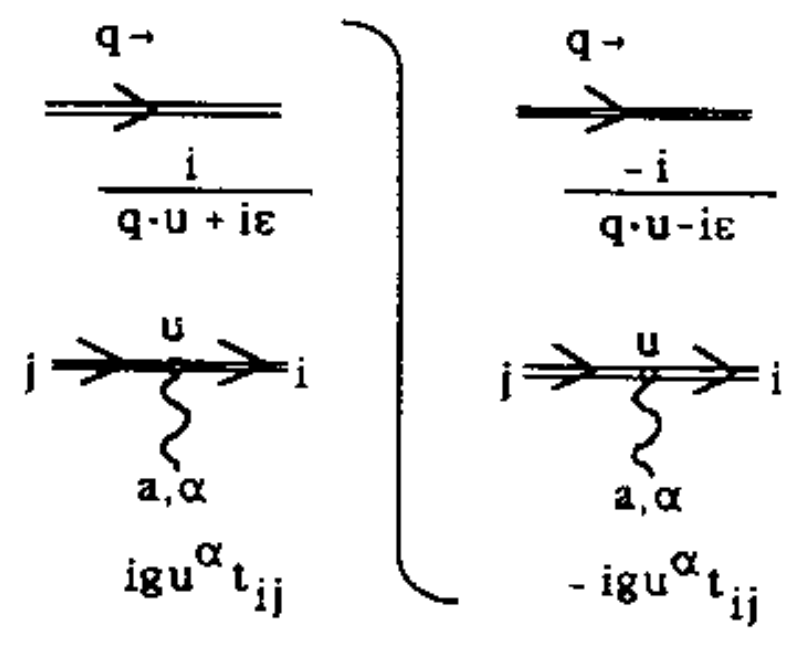
\includegraphics[width=0.8\textwidth]{feyn}
		\end{column}
		\begin{column}{.5\textwidth}
			\begin{itemize}
				\item One can read off the Feynman rules from the expansion.
				\item The \alert{denominators} are represented by double lines, which we shall refer to \textbf{eikonal} lines
				\item They attach to the gluon propagator via a vertex proportional to $-ign^\mu$
			\end{itemize}
		\end{column}
	\end{columns}
\end{frame}

\subsection{Renormalization}

\begin{frame}{Renormalization}
	The function $f_{i/A}(\xi)$ is \textbf{unrenormalized}, being defined using bare fields, a bare coupling, bare parton masses ... and so on
	\begin{itemize}
		\item would like to introduce the $\overbar{MS}$ scheme
		\item perform integration in $4-2\epsilon$ dimensions, including a factor that keeps the dimension constant
	\end{itemize}\vskip0.15in

	\begin{block}{Renormalized, gauge invariant definition of $f_{i/A}(\xi,\mu)$}
		\begin{align*}
			f_{i/A}(\xi,\mu) = \frac{1}{4\pi} \int \dif y^- e^{-i\xi P^+ y^-} \braket{P|  \overbar{\psi}_i(0,y^-,\mathbf{0})\gamma^+\mathcal{O}(y^-,0)\psi_i(0) |P}_{\tiny\overbar{MS}}\\
		\end{align*}
	\end{block}
\end{frame}

\begin{frame}{Antiquarks and Gluons}
	Will simply state results ... \vskip0.15in
	\begin{itemize}
		\item Antiquarks : utilize charge conjugation, $\overbar{\mathbf{3}}$ representation generators for $\mathcal{O}$
		\begin{align*}
			f_{i/A}(\xi,\mu) = \frac{1}{4\pi} \int \dif y^- e^{-i\xi P^+ y^-} \braket{P|\text{Tr}\left[\gamma^+ \psi_i(0,y^-,\mathbf{0})\mathcal{O}(y^-,0)\overbar{\psi}_i(0) \right]  |P}_{\tiny\overbar{MS}}
		\end{align*}
		\item Gluons : $A^+=0$ gauge, $\mathbf{8}$ representation generators for $\mathcal{O}$
		\begin{align*}
			f_{g/A}(\xi,\mu) = \frac{1}{2\pi x P^+} \int \dif y^- e^{-i\xi P^+ y^-} \braket{P|F^+_a(0,y^-,\mathbf{0})^\nu \mathcal{O}_{ab} F^+_b(0)^\nu|P}_{\tiny\overbar{MS}}
		\end{align*}
	\end{itemize}
\end{frame}

\begin{frame}{Renormalization Group}
	\begin{itemize}
		\item A change in the scale $\mu$ affects $f_{a/A}(\xi,\mu)$, which comes from the change in the amount of UV divergence that renormalization is removing.
		\item By examining the structure of UV divergences, one finds $f_{a/A}(\xi,\mu)$ obeys DGLAP evolution equations,
		\begin{align*}
			\mu^2 \dder{}{ \mu^2} f_{a/A}(\xi,\mu) = \sum_b \int_{\xi}^1 \frac{\dif z}{z} P_{ab}(z,\alpha_S(\mu^2))f_{b/A}(\xi/z,\mu)
		\end{align*}
		\setbeamertemplate{itemize items}[triangle]
		\begin{itemize}
			\item The evolution kernels $P_{ab}$ are perturbatively calculable as expansions in powers of $\alpha_S(\mu)$
			\item Exact evolution kernels have been known up to NNLO (2004), 
		\end{itemize}
	\end{itemize}
\end{frame}

\begin{frame}{Renormalization Group}
	Interpretation? The parameter $\mu$ corresponds to the physical resolving power of the probe.\vskip0.1in
	\begin{itemize}
		\item Parton splitting is not well observed at low resolving power
		\item At higher $\mu$ which is enough to resolve mother parton into its daughters, observing a splitting
	\end{itemize}
	\begin{columns}[T]
		\begin{column}{.5\textwidth}
			\begin{figure}
				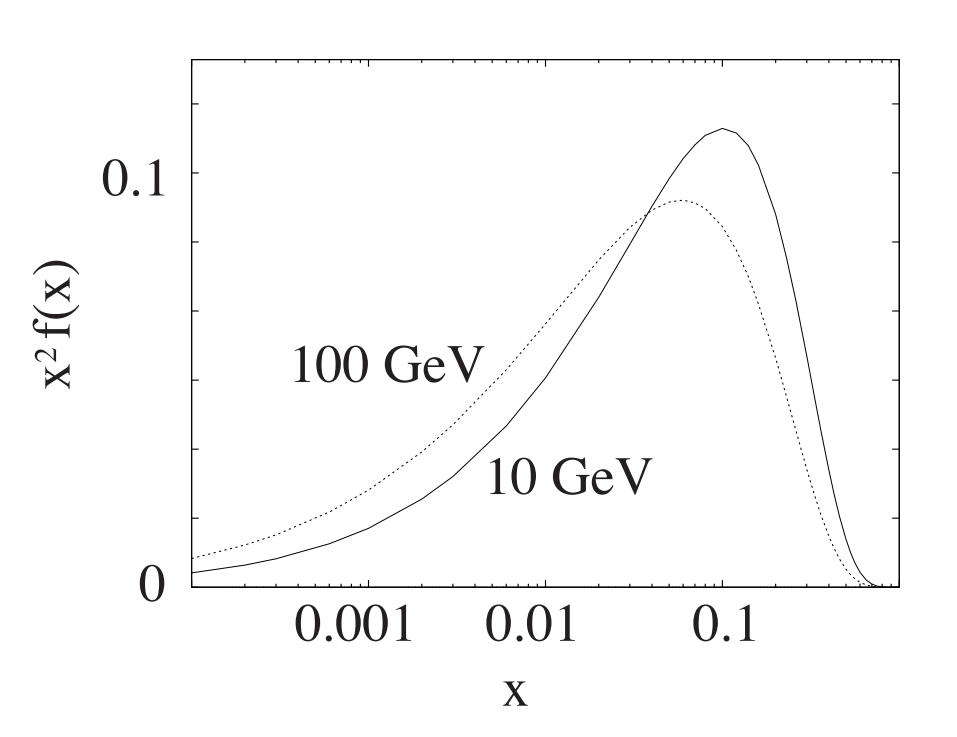
\includegraphics[width=.75\textwidth]{evol}
			\end{figure}
		\end{column}
		\begin{column}{.5\textwidth}
			\setbeamertemplate{itemize items}[triangle]
			\begin{itemize}
				\item One can find parton distributions at $\mu$ when it is already known at $\mu_0 < \mu$, using the RG equation.
				\item Gluon distribution at $\mu=10,100$ $GeV$ using the CTEQ3M PDF set
				\item With greater resolution, smaller momentum fraction due to parton splitting.
			\end{itemize}
		\end{column}
	\end{columns}
\end{frame}
%------------------------------------------------

%\begin{frame}{Translation to local operators}
%	We've defined PDFs as hadron matrix elements of a certain operator, which is not local but \textbf{bilocal}, along the light-like line.
%	\setbeamertemplate{itemize items}[triangle]
%	\begin{itemize}
%			\item Let us relate PDFs to products of operators all at the same point, in a \textbf{local} sense. 
%		\item Has computational advantages; evaluation of bilocal operators would be difficult in lattice QCD ...
%	\end{itemize}\vskip0.1in

%\begin{columns}[T]
%	\begin{column}{.5\textwidth}
%		According to the previous definitions,
%		\begin{itemize}
%			\item $f_{j/A}(\xi,\mu)=0$ for $\xi>1$
%			\item $f_{\bar{j}/A}(\xi,\mu)=0$ for $\xi>1$
%			\item $f_{j/A}(\xi,\mu) = - f_{\bar{j}/A}(\xi,\mu)$
%		\end{itemize}
%	\end{column}
%	\begin{column}{.5\textwidth}
%		Consider the moments of the quark/antiquark distributions d%efined as
%		\begin{align*}
%			M_j^{(J)}(\mu) = \int_0^1 \frac{\dif \xi}{\xi} \xi
%		\end{align*}
%	\end{column}
%\end{columns}
%
%	
%\end{frame}

%\section{Fitting PDFs}

%\subsection{Importance of PDF Fitting}
%\begin{frame}{}
%	content...
%\end{frame}

\begin{frame}{Summary}
	\begin{itemize}
		\item PDFs can be constructed as a hadron matrix
		element of the number density operator for quarks.
		\item PDFs should be renormalized due to divergences from NLO and beyond.
		\item Renormalization scale corresponds to the physical resolving power of the probe.
	\end{itemize}
\end{frame}

\begin{frame}
    \Huge{\centerline{Thank You}}
\end{frame}

%----------------------------------------------------------------------------------------

\end{document}